\documentclass[12pt, letterpaper]{article}

\title{My First Latex Document}
\author{Rana Universe\thanks{Mail Us AT: RanaUniverse321@gmail.com}}
\date{August 2025}


\usepackage{lipsum}

\usepackage{graphicx} %LaTeX package to import graphics
\graphicspath{{images/}} %configuring the graphicx package

% \renewcommand{\figurename}{Graph Image}
% To get Figure 1,2,3... i will use normal, if i want custom name i will uncomment this upper, which will say, Graphh Image 1, 2, 3 ...


\usepackage{pgffor} % For loops i will use this package so that i can use repetative work easily






\begin{document}
\maketitle






\begin{figure}[htbp]
\centering

\fbox{

\includegraphics[width=0.5\textwidth]{rana_universe_logo_round_black.png}
}

\caption{Rana Universe logo in black circle}

\label{fig:rana-logo}

\end{figure}



\newpage

\foreach \name in {Rana, Universe, RanaUniverse} {
    Hello, \name! \par
}


\vspace{5em}
\foreach \n in {1,...,9} {
    I am Rana Universe...(\n) \par
}

\vspace{3em}

\foreach \n in {1,...,9} {
    \noindent \textbf{\n.} I am Rana Universe... \par

    \textbf{\n.} I am Rana Universe... \par
}



\begin{figure}[ht]   % Start figure environment
    \centering   % Center the image

    % 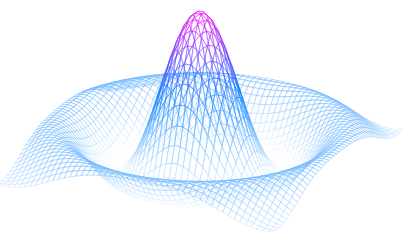
\includegraphics[width=.5\textwidth]{mesh.png}    

    % This below is for adding a black border
    \fbox{
        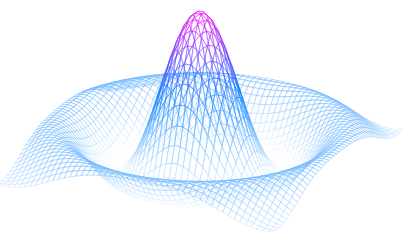
\includegraphics[width=0.5\textwidth]{mesh.png}
    }

    \caption{\textbf{A nice plot.}}   
    \label{fig:mesh1}   % Label: Internal name used to reference the figure, it should be unique
\end{figure}


As you can see in \textbf{Figure \ref{fig:mesh1}}, the function grows near the origin. This example is on page \pageref{fig:mesh1}.


As you can see in \textbf{\textit{Figure \ref{fig:mesh1}}}, the function grows near the origin. This example is on page \pageref{fig:mesh1}.



\begin{figure}[htbp]
	\centering
	
\includegraphics[width=0.5\textwidth]{linux_logo.png}
	\caption{\textbf{Linux Logo}}
	\label{fig:linuxlogo}
\end{figure}

Now in \textit{Figure \ref{fig:linuxlogo}}, you can see the famous Linux logo.
This is shown on page \pageref{fig:linuxlogo}.





\vspace{10em}

I am Rana Universe...

I am Rana Universe...

I am Rana Universe...

I am Rana Universe...

I am Rana Universe...

I am Rana Universe...

I am Rana Universe...

I am Rana Universe...

I am Rana Universe...

\vspace{3em}





\lipsum[1]

\lipsum[2]

\vspace{1em}

\lipsum[1]




% This line here is a comment. It will not be typeset in the document.
\end{document}



